\chap{Team Work}

\section{How we apply Agile process}
\vspace{-5mm}
As Agile is based on iterations, this project has been organized in three of them. During each iteration, the \textit{plan-design-built-try} process has been developed in the best way possible, learning from errors and tried to improve the process from one iteration to another.
	\subsection{First iteration}
	\vspace{-5mm}
	We started the project deciding \textbf{what} we wanted to do; the aim of the application. We also decided that the first iteration should be for the general structure of the platform: main page, basic static pages and basic functionality. For designing, we draw the different pages and how they should look, behave and connect between them. Also, we decided and did a schema of the structure of the models (see Figure \ref{fig: Models}).\\
	After design the basic structure, we did the user stories for that structure in a shared document (via \href{https://drive.google.com/drive/my-drive/}{Google Drive}). For example:
	\begin{itemize} \setlength{\itemsep}{-5pt}
	\item As a public user, I’ll be able to reach the web application site. 1 point
	\item As a public user, I’ll need to be able to create a private user. 5 points
	\item As an admin, I’ll be able to see the list of users. 5 points
	\end{itemize}
	For coding, this iteration was the most difficult one, as far as we had to learn Ruby on Rails from the very beginning. For the first steps, we used \href{https://www.railstutorial.org/book/}{a Ruby tutorial} which help us to learn how to start a project in Rails.\\
	Due to the hard start, we ended the first iteration doing around 80\% of the user stories we had at the beginning. Thus, we re-scheduled the work plan, checking which worked and which did not.
	\subsection{Second iteration}
	\vspace{-5mm}
	We started this with the basic structure implemented; we planned the amount of work we could face in the time we had and did the corresponding user stories. This time, we tried to be more effective and organized and started to use \textit{Pivotal Tracker} for user stories. The improvement of using this platform instead of \textit{Google Drive} is explained in Section \ref{Pivotal_Tracker}.\\
	The objective of this iteration was to do the real implementation of the application. That is, all the functionality of the platform, as we had thought it in the beginning. We re-planned (and draw it again) the pages, but this time with the non-basic behaviour we wanted. For example, this was the time for implement the ability of an user of joining a timetable, or for letting a timetable to have several events.\\
	In terms of coding, that meant ending the database and relationships between the models, and being used to the capacities of Ruby on Rails. The most powerful tool of Ruby we found is the use of foreign keys; the way you can pass though all the models in one variable, and the capacity of mixing html with Ruby's code.\\
	Even though we couldn't achieve all the implementation scheduled, we did almost everything and had to re-plan just a few things for the third and last iteration. In order to plan it properly, we did a document with all the errors or bad behaviours we could find. This document was not unique, but was for re-writing it while we used more and more the application, during the whole third iteration.
	\subsection{Third iteration}
	\vspace{-5mm}
	The work planned for this one was separated in three parts: 1) to end with the re-scheduled work from iteration two (e.g. the contact form); 2) to do the graphics of the website and 3) going through the app and fix all the small "problems" (e.g. a problem with the admin page, or a missing \textit{Help} link). As before, we used Pivotal Tracker for the user stories, for being conscious of the remaining work. During this iteration, we did "small" agile iterations, due to the fact we were fixing problems and redoing the code. \\
	We ended the iteration with the application working properly (except a graphic issue in the about page) and all the expected functionality implemented.
	
\section{Team cooperation and communication}
\vspace{-5mm}
Promote cooperation and communication between team members is probably one of the most important thing during a group project development process. Most of the time it's hard to figure out a good way for cooperate and communicate between each other, and also during this project it has been an relative issue, in particular in the first part of the project. It was mainly caused by different schedules, lectures and available time of each member of the team.
Even that, every single team member agreed about the importance of frequent meetings, so we almost always planned a group meeting once per week. 
The main communication way between the team member has been a chat group: it was used for decide team meeting and also to update the other teams about ideas or news about the code.
We basically spent the meeting's time:
\vspace{-5mm}
\begin{itemize}
 \setlength{\itemsep}{-5pt}
 \item Helping each other with any kind of problems about the project.
 \item Discussing new ideas.
 \item Planning what to do in the following period.
\end{itemize} 
\vspace{-5mm}

\section{Instruments and Applications usage}
\vspace{-5mm}
	\subsection{Git}
	\vspace{-5mm}
During the whole project development \textbf{Git} has been an indispensable instrument.\\
It is possible to define Git as a version control system, which means that the principal purpose is to help a software team manage changes to source code over time. In particular, it keeps track of every modification to the code in a special kind of database and, if a mistake is made, developers have the possibility to turn back and compare earlier version of the code in order to fix the mistake.\cite{versionController}\\
During this project, Git usage has been improved a lot between the first iteration and the last one. For example, during the first part of the project there were several problems about merging and push/pull of code, mainly caused by a lack of knowledge about how to use this system in a proper way. Then, once learnt from our mistakes, during the following parts of the project Git usage has been improved a lot and it provided a significant help to the team work. Probably the most appreciated Git function during this project was the possibility to always check out the latest version of the code, since all the team members were committing code quite often.

	\subsection{Pivotal Tracker} \label{Pivotal_Tracker}
	\vspace{-5mm}
As we have explained before, we did user stories in a shared document in the first iteration; it resulted not very productive. Thus, we looked for some tool to improve the usefulness of user stories. We found \href{https://www.pivotaltracker.com/}{Pivotal Tracker}, a website that let you start a project and add user stories to it. They have the format before explained (see Section \ref{Agile}), and also let you give each story Fibonacci points. Furthermore, it let you add different tasks to each story, which makes very easy to schedule your work and to see others' progress. Also, a person can "choose" a task, and marked it as \textit{started}, thus others would know which tasks have already a "owner".
\begin{figure}[H]
	\centering
	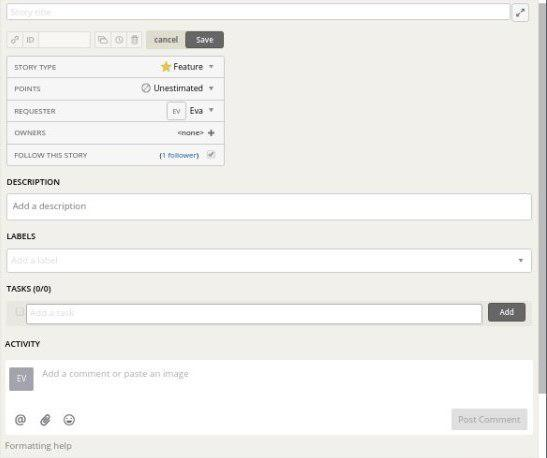
\includegraphics[trim={0 0 0 0},clip,width=1\textwidth]{Files/user_story.jpg}
	\caption{User Story from Pivotal Tracker}
	\label{fig: MVC}
\end{figure}

